\documentclass[11pt]{article}

\usepackage[a4paper, margin=1in]{geometry}
\usepackage{amsmath, amssymb}
\usepackage{graphicx}
\usepackage{biblatex}

\addbibresource{refs.bib}

\title{Camp Project Markov Chain}
\author{Hope Coltrin}
\date{\today}

\begin{document}

\maketitle

\begin{abstract}
This project uses a Markov chain to simulate a sequence of
states, and I compare the empirical frequency of each state I found with its
stationary distribution.

\end{abstract}

\section{Introduction}

A Markov chain is a process where the next state depends on the current
state through probabilities of each transition. These models can be used throughout economics. Athreya and Majumdar (2003) study estimation of the stationary distribution of a Markov chain \parencite{athreya2003markovchain}.

In this project, I simulate a two-state Markov chain to check if the empirical frequency approaches the stationary distribution in the long run.

\section{Model}

The transition matrix I used in the simulation is

\[
P =
\begin{pmatrix}
0.8 & 0.2 \\
0.3 & 0.7
\end{pmatrix}.
\]

Each row sums to one. The stationary distribution is the long run distribution of states that never changes between transitions. Seen in this equation:

\[
\pi P = \pi.
\]

For this transition matrix, the stationary probabilities are

\[
\pi_0 =
\frac{0.3}{0.2+0.3} = 0.6,
\qquad
\pi_1 =
\frac{0.2}{0.2+0.3} = 0.4.
\]

The empirical frequency should get closer to these probabilities as
the number of periods increases.

\section{Results}

I simulated the path of a long run transition matrix. Figure~\ref{fig:convergence}
shows the results.

\begin{figure}[ht]
\centering
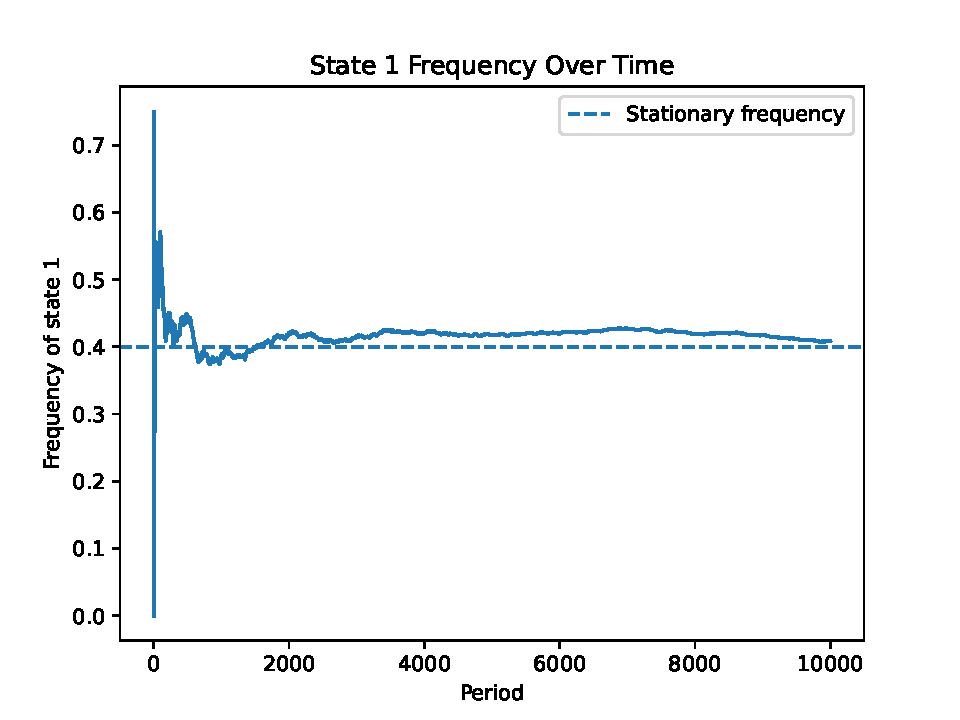
\includegraphics[width=0.7\linewidth]{figures/convergence.pdf}
\caption{The frequency of state 1 over time is shown. The dashed line shows the stationary probability.}
\label{fig:convergence}
\end{figure}

The running frequency moves toward the stationary probability as the number of rounds, showing convergence to the stationary distribution.

\printbibliography

\end{document}